\chapter{Samplers: Framework Android}

\section{Propuesta general}

\subsection{Descripción del problema}

Como se vio antes, se necesitaba de un entorno que permitiera a un científico poder crear una aplicación móvil con facilidad para poder incluir ciencia ciudadana en sus proyectos de ciencia ciudadana, mas precisamente, en proyectos de recolección.

La idea es que un científico pueda crear una aplicación móvil de ciencia ciudadana sin tener conocimientos de programación. Por ejemplo, desde una página web armar el protocolo de recolección de las muestras y con el mismo poder generar una aplicación móvil que sirva para tomar las muestras siguiendo dicho protocolo.

El protocolo de recolección estaría compuesto por los diferentes pasos necesarios para tomar la muestra con la aplicación. Estos pasos deben permitir:
\begin{itemize}
\item capturar una foto, un video o un audio.
\item tomar la posición del GPS o grabar un recorrido con el GPS.
\item contestar una pregunta con respecto a la muestra. Esta pregunta puede tener una o múltiples respuestas posibles.
\item introducir anotaciones (texto).
\item seleccionar una fecha o una hora.
\item mostrar información de orientación para la toma de la muestra.
\end{itemize}

Las muestras recolectadas con la aplicación deben ser enviadas por Internet a un servidor web previamente configurado para dicho propósito.

La aplicación generada debe ser una aplicación nativa, y no una solución web por ejemplo, para poder aprovechar mejor las características de los dispositivos móviles (cámara, GPS, etc.). Además se debe contemplar que al momento de tomar una muestra es posible que no se cuente con conexión a Internet, pero igualmente se debe permitir la toma de la muestra y se la debe almacenar en el dispositivo móvil hasta que haya conexión a Internet y pueda ser enviada al servidor web.

La aplicación generada servirá para tomar muestras siguiendo el protocolo de recolección especificado, almacenarlas y empaquetarlas en el dispositivo móvil hasta que puedan ser enviadas al servidor web.

Además se deberá contemplar algún mecanismo para poder mostrar ayuda para el usuario final de la aplicación (el científico ciudadano) que sirviera de orientación para tomar la muestra. 

También se debe contemplar algún mecanismo de identificación del usuario que toma las muestras, con usuario y contraseña, o con alguna red social (Facebook, Twitter, Instagram, Google, etc.) para así poder darle una devolución mostrándole información, o incentivarlo para que siga participando del proyecto a través de gamificación por ejemplo.



\subsection{Alcance de la solución propuesta}
En un principio, Samplers se pensó para que un científico pudiera crear su propia aplicación móvil de ciencia ciudadana sin tener conocimientos de programación. 
La idea inicial era que, mediante una aplicación web, el científico pudiera armar el protocolo de recolección de las muestras de manera visual e intuitiva, y se generara un archivo de configuración para Samplers. 
Con el archivo de configuración se pasaría a Samplers y se generaría la app para Android (el archivo APK para instalarla). 
Pero de esta forma el alcance de la tesis era muy grande, por lo que se decidió quitar la parte de la aplicación web y suponer que que el archivo de configuración ya viene armado.

Como se mencionó antes se requerían aplicaciones nativas, pero abarcar los 3 sistemas operativos móviles más usados en ese momento (Android, iOS y Windows Phone) era mucho para el alcance de esta tesis, por lo que se decidió optar por Android, que era el sistema operativo móvil más usado en ese momento. Según una estadística de Gartner sobre las ventas de smartphones a nivel mundial en el último trimestre de 2016\cite{gartner}, mas del 80\% de las mismas fueron de celulares con Android, y ese porcentaje fue creciendo hasta obtener una cuota del mercado del 88\% a nivel mundial a mediados de 2018. En la actualidad, en Argentina esa cuota de mercado es mas grande, llegando al 93\% según datos publicados por Carrier y Asociados en su reporte Mercado Celular Argentino 2019\cite{carrier}.

Para desarrollar aplicaciones móviles para la plataforma Android, el entorno de desarrollo integrado (IDE por sus siglas en inglés) oficial es Android Studio\cite{androidStudio}, por lo que Samplers se apoya sobre el mismo. Android Studio ha sido publicado de forma gratuita bajo Licencia Apache 2.0 y está disponible para las plataformas Microsoft Windows, MacOS y GNU/Linux.

\subsection{Descripción de la solución propuesta: Samplers}
Samplers es un framework que permite construir, de manera sencilla, aplicaciones Android (apps) para recolectar muestras en proyectos de Ciencia Ciudadana. Brinda una solución simple al problema de la recolección de la muestra aprovechando las funcionalidades de los dispositivos móviles.

Configurando el Workflow (que representa el protocolo de recolección en Samplers) y unos parámetros más, con Samplers se puede generar una app lista para ejecutarse en un dispositivo móvil Android. Esta app generada sirve para tomar muestras siguiendo el Workflow especificado, y las almacena en el dispositivo móvil hasta que puedan ser enviadas a un servidor web previamente configurado.

La app generada contiene, entre otras cosas, una Activity principal que muestra un texto de bienvenida (configurable) y un botón para tomar una muestra. Al presionar dicho botón se llama a la Activity encargada de tomar las muestras siguiendo el Workflow configurado. Esta Activity va mostrando en pantalla un Fragment por cada «paso» dentro del Workflow (Steps en Samplers). Cada uno de estos Fragments va interactuando con el usuario final de la app, el científico ciudadano\footnote{Se diferencia al usuario de Samplers, que es el que desea generar una app para recolectar muestras en un proyecto de ciencia ciudadana, del usuario final de la app, que es quien va a usar la app generada, que sería el científico ciudadano.}, para completar cada uno de los Steps del Workflow y así tomar la muestra (Sample en Samplers).

Para configurar el Workflow y los demás parámetros que necesita Samplers para generar la app, se debe completar un archivo de configuración llamado SamplersConfig.json.

Por ejemplo, si se desea crear una aplicación para hacer un relevamiento de las zonas con presencia del mosquito transmisor del Dengue (Aedes Aegypti), solicitando a los científicos ciudadanos que tomen fotos de los mosquitos que encuentren con las características del mosquito Aedes Aegypti, junto con la posición del GPS del dispositivo móvil. De esta manera se podría identificar al mosquito con la foto, y con la posición GPS armar un mapa de los avistajes. Para recolectar estas muestras se podría definir el protocolo de recolección de la siguiente manera:

\begin{enumerate}

\item Mostrar al científico ciudadano las características del mosquito Aedes Aegypti para que las pueda comparar con el mosquito encontrado (para evitar el envío de fotos innecesarias).

\item Pedir al científico ciudadano que tome una foto desde arriba del mosquito.

\item Pedir al científico ciudadano que tome una foto del costado del mosquito.

\item Pedir al científico ciudadano que tome la posición del GPS

\end{enumerate}

Para representar este protocolo de recolección se debería configurar el Workflow en el archivo de configuración para Samplers de la siguiente manera: 

\begin{figure}[H]
  \centering
    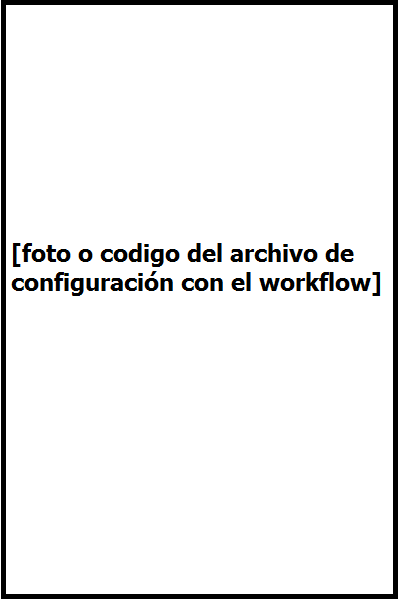
\includegraphics[scale=0.8]{05-implementacion/archivo_config_ejemplo.png} 
   \caption{Archivo de configuración para Samplers de la app ejemplo}
\end{figure}


Con este archivo de configuración, Samplers generará el código necesario para la app, que al compilarla y ejecutarla en un dispositivo móvil Android se verá como muestra la siguiente imagen:


\begin{figure}[H]
  \centering
    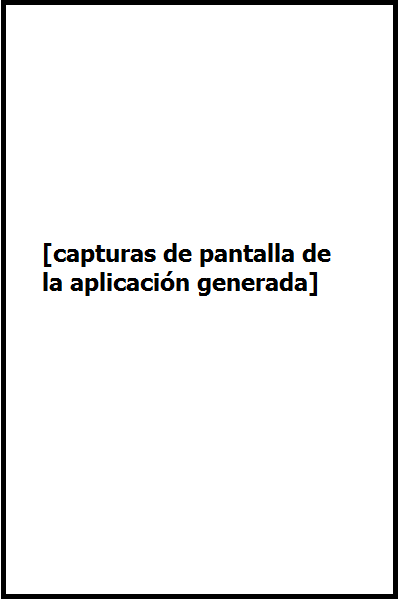
\includegraphics[scale=0.8]{05-implementacion/app_generada_ejemplo.png} 
   \caption{Capturas de pantalla de la app de ejemplo generada por Samplers}
\end{figure}


Las opciones disponibles y cómo se configura el archivo de configuración de Samplers se explican en la sección \ref{sec:archivo_configuracion}.

De esta manera un científico que desee generar una app para su proyecto de ciencia ciudadana, solo tiene que completar el archivo de configuración, ejecutar Samplers y luego compilar en Android Studio y ejecutar la app en un dispositivo móvil o en los dispositivos virtuales que provee Android Studio para debugging.

Como Samplers genera el código fuente de la app, esto permite que un usuario con conocimientos de programación pueda modificarlo y personalizar la app a su gusto, así como también agregarle otras funcionalidades a la app generada. También permite que pueda ser usado en una app ya desarrollada o en desarrollo, como si fuera una librería que se incluye al proyecto y permite usar sus clases (esto se explica con más detalle en la sección \ref{sec:usando_las_clases}).

Como Samplers se pensó como un proyecto dentro de Cientópolis\cite{cientopolis} el mismo es open source y se usó un repositorio público en GitHub\cite{github} para dejar el código fuente disponible para todo el mundo.


\begin{comment}
También provee un mecanismo de identificación del usuario final de la aplicación (el científico ciudadano) usando su cuenta de Google, ya que en los dispositivos móviles con sistema operativo Android se requiere de una cuenta de Google para acceder a muchas de las funcionalidades, como por ejemplo la Play Store (la tienda de Android para descargar aplicaciones).  Ademas esta preparado para que el usuario del framework pueda incluir su propio sistema de inicio de sesión (por ejemplo con usuario y contraseña) o con una API de alguna red social, como Facebook, Twitter, Instagram, etc.


Samplers también provee un mecanismo para mostrar ayuda asociada a un paso (Step) en particular y una ayuda general en la pantalla principal, usando archivos HTML. Se optó por los mismos por la variedad de opciones y posibilidades que conllevan, y por su simpleza para mostrarlos.
\end{comment}

\section{Archivo de configuración}\label{sec:archivo_configuracion}

\begin{comment}

En el objeto project, se encuentran las configuraciones del proyecto de Android Studio en el cual se creará la app, y son las siguientes:
\begin{itemize}

\item app\_path: la ruta relativa a los archivos fuente de la app. Es donde se crearán los archivos de las Activities por ejemplo.

\item package\_name: el nombre del package que se usará para las Activities de la app (generalmente ``com.example.myApplication"). 

\end{itemize}

En el objeto application, se encuentran los parámetros para configurar la app, como por ejemplo el mensaje de bienvenida o el servidor web al que se deben enviar las muestras recolectadas. Los parámetros son los siguientes:
\begin{itemize}

\item title: el título de la app.

\item welcomeMessage: el mensaje de bienvenida que se muestra en la Activity principal.  

\item networkConfiguration: la configuración del servidor al que se enviarán las muestras tomadas con la app

\begin{itemize}
\item url: la url del servidor a la cual se enviarán las muestras mediante un mensaje HTTP POST.

\item paramName: el nombre del parámetro dentro del mensaje HTTP POST que se usará para enviar la muestra.

\item paramNameUserId: [Opcional] el nombre del parámetro dentro del mensaje HTTP POST que se usará para enviar el id del usuario que tomó la muestra (si los métodos de identificación estan habilitados).

\item paramNameAuthenticationType: [Opcional] el nombre del parámetro dentro del mensaje HTTP POST que se usará para enviar el tipo de identificación que se usó (si los métodos de identificación estan habilitados).

\end{itemize}

\item googleMaps\_API\_KEY:

\item mainHelpFileName: [Opcional] se puede espe 
el nombre del archivo HTML que se usará.
The file name of the HTML file containing the main application help

\item authenticationEnabled: [Opcional] habilita los métodos de identificación del usuario que toma las muestras.

\item authenticationOptional: [Opcional] indica si la identificación (en caso de estar habilitada) será opcional u obligatoria.


\end{itemize}

\end{comment}

El archivo de configuración es un archivo en formato JSON que se debe completar con los parámetros necesarios para crear la app con Samplers. Se eligió el formato JSON porque nos pareció más sencillo de manipularlo por una persona (que XML por ejemplo, que también fue evaluado), suponiendo que el científico tuviese que editarlo manualmente.

El archivo está compuesto por tres objetos: project, application y workflow.

En el objeto project, se encuentran las configuraciones del proyecto de Android Studio en el cual se creará la app, como por ejemplo la ruta en donde se crearán los archivos de las Activities y el nombre del package que se usará para las mismas. 

En el objeto application, se encuentran los parámetros para configurar la app, como por ejemplo el título de la app, el mensaje de bienvenida o el servidor web al que se deben enviar las muestras recolectadas. 

El objeto workflow se usa justamente para configurar el Workflow (el protocolo de recolección) que usará la app para tomar las muestras. En el mismo se deben especificar los Steps que se usarán con sus respectivos parámetros cada uno. Por defecto Samplers provee los siguientes Steps:

\begin{itemize}

\item Information: Muestra un texto al científico ciudadano.

\item Photo: Solicita tomar una foto.

\item Sound: Solicita grabar sonido.

\item Location: Solicita tomar la posición del GPS del dispositivo móvil.

\item Route: Solicita grabar con el GPS del dispositivo móvil un recorrido (un conjunto de posiciones GPS).

\item SelectOne: Solicita seleccionar una única respuesta a una pregunta.

\item MultipleSelect: Solicita seleccionar una o varias respuestas a una pregunta.

\item InsertText: Solicita ingresar texto.

\item InsertDate: Solicita seleccionar una fecha.

\item InsertTime: Solicita seleccionar una hora.

\end{itemize}

En la siguiente imagen se muestra un ejemplo del archivo de configuración para Samplers.
\begin{figure}[H]
  \centering
    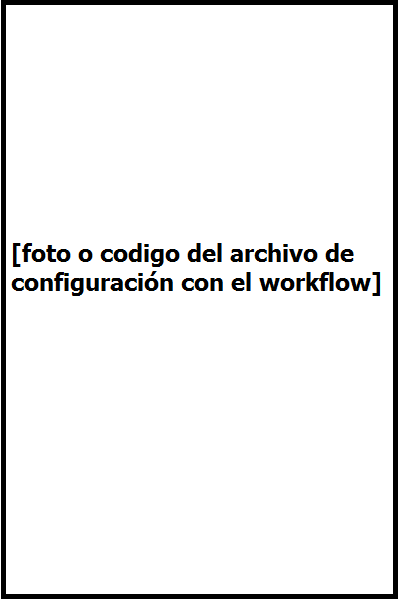
\includegraphics[scale=0.8]{05-implementacion/archivo_config_ejemplo.png} 
   \caption{Ejemplo de un archivo de configuración para Samplers}
\end{figure}

Una vez configurado el archivo, Samplers generará una Activity principal para la app que tendrá todas las configuraciones del objeto application y que usará el Workflow configurado para llamar a la Activity encargada de tomar las muestras (TakeSampleActivity) cuando el científico ciudadano presione el botón para tomar una muestra.

El detalle de todos los parámetros, como configurar el archivo de configuración y los diferentes Steps disponibles para armar el Workflow se explican en la sección \ref{sec:archivo_config_detallado}


\section{Usando las clases} \label{sec:usando_las_clases}

[Aca explicaremos cómo sería usando las clases (para una app existente por ejemplo), pero sencillo y por arriba porque todavia no se explicaron las clases en detalle que viene en la siguiente sección].

\section{Estructura del Framework}
Samplers está compuesto por dos elementos: una librería con las clases y [demases (activities, fragments, recursos)] necesarias para crear la app y un script en Gradle para procesar el archivo de configuración.

A continuación se explican las clases que permiten que se cree una aplicación móvil con Samplers y su funcionamiento.

\subsection{Workflow, Step, StepFragment, StepResult, Sample}
Estas clases conforman el corazón del framework, y son las necesarias para poder definir el protocolo de recolección de las muestras.

A continuación se muestra el diagrama de clases (Figura \ref{fig:umlFrameworkCore}).

\begin{figure}[H]
  \centering
    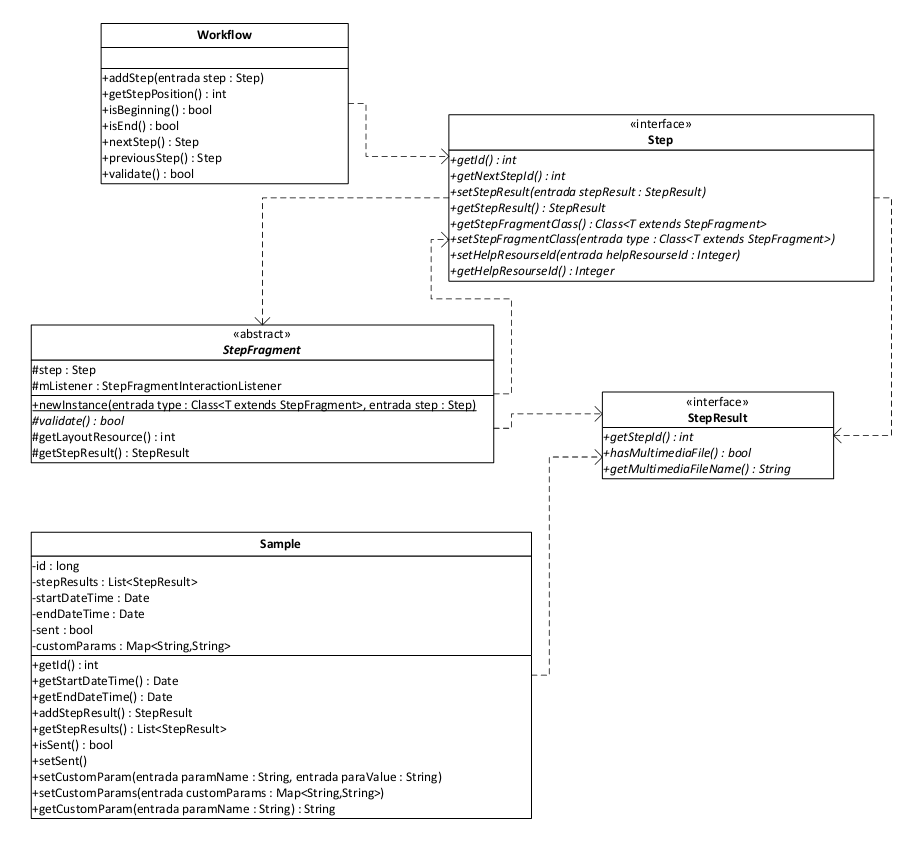
\includegraphics[scale=0.4]{05-implementacion/FrameworkCore.png} 
   \caption{Diagrama de clases del core del framework}
   \label{fig:umlFrameworkCore}
\end{figure}

\begin{comment}
TakeSampleActivity es una Activity encargada de tomar la muestra.
Recibe como parámetro un Workflow, que representa el protocolo de recolección de la muestra.
El Workflow esta formado por varias instancias de Step, que representan cada una un paso a seguir dentro del protocolo de recolección para obtener la muestra.

TakeSampleActivity ejecuta el Workflow y por cada Step obtiene y muestra en pantalla el StepFragment asociado, que es el Fragment encargado de mostrar la interfaz de usuario para ejecutar ese Step. 
El StepFragment a través de la interacción con el usuario final (el científico ciudadano) genera un StepResult, que es el resultado de la ejecución del Step asociado. Por cada tipo de Step, debe haber una clase StepFragment que sepa ejecutar ese Step y generar el StepResult asociado

El conjunto de todos los StepResults obtenidos después de ejecutar todos los Steps del Workflow forman la muestra, que esta representada por la clase Sample.

TakeSampleActivity genera una muestra (sample)
\end{comment}


\subsubsection{Workflow: el protocolo de recolección de las muestras}
La clase Workflow representa el protocolo de recolección de las muestras. Está formado por una colección de Steps, que representan los pasos a seguir para completar dicho protocolo, y un Step inicial que indica el inicio del mismo (el primer Step a ejecutar).

El Workflow es el encargado de llevar el estado del paso en el que se encuentra, y posee métodos para obtener el siguiente Step (\textit{nextStep()}  que depende del Step actual) y el Step anterior (\textit{previuosStep()}  para lo que maneja una lista a modo de pila\footnote{Stack en inglés, una lista ordenada con acceso a sus elementos de tipo «último en entrar, primero en salir»}).

El Workflow se comporta de manera secuencial, puede ir hacia adelante o volver hacia atrás, pero esto no impide que pueda tener bifurcaciones, y así formar diferentes caminos para tomar la muestra. Por ejemplo, se le podría preguntar al científico ciudadano si observa una característica particular al momento de tomar la muestra, y si la observa solicitarle que tome una foto de la misma, pero en caso contrario se puede omitir el paso de la foto.

\subsubsection{Step: el paso}
Un Step representa un paso dentro del Workflow.

\begin{comment}
*** ACA FALTA CORREGIR  ***
\end{comment}

Se definió como una interfaz, ya que su comportamiento depende de la implementación de cada tipo de Step que se defina. Con esto también se evita que los Steps creados por los usuarios programadores tengan que heredar de una clase en particular, y solo necesiten implementar la interfaz.

El Step tiene asociado un StepFragment (la vista y controlador) que es el encargado de ejecutar el Step para generar un resultado (StepResult). El Step básicamente tiene los parámetros o información para que pueda ser ejecutado por el StepFragment, y no tiene mucho comportamiento.

Por ejemplo, para el caso en que el paso sea contestar una pregunta, el Step tendrá la pregunta en sí (un String) y una colección con las posibles respuestas (id y descripción).

El Step conoce cuál es el siguiente Step a ejecutar aunque a veces éste depende del StepResult generado, como es el caso de SelectOneStep en el que el siguiente paso depende de la opción seleccionada, y con esto se pueden crear bifurcaciones en el Workflow.

Samplers provee los siguientes Steps:
\begin{itemize}
	\item InformationStep: Muestra una información (texto) al usuario.
	\item PhotoStep: Permite tomar una foto con la cámara del dispositivo móvil.
	\item SoundRecordStep: Permite grabar un sonido con el micrófono del dispositivo móvil.
	\item SelectOneStep: Muestra una pregunta con varias opciones como respuesta, de las cuales solo se puede seleccionar una sola.
	\item MultipleSelectStep: Muestra una pregunta con varias opciones como respuesta, de las cuales solo se pueden seleccionar varias opciones.
	\item LocationStep: Permite tomar la geo posición del dispositivo móvil.
	\item RouteStep: Permite grabar un recorrido usando el GPS del dispositivo móvil.
	\item InsertTextStep: Permite ingresar un texto.
	\item InsertDateStep: Permite seleccionar una fecha.
	\item InsertTimeStep: Permite seleccionar una hora.
\end{itemize}

El detalle de estos Steps y su funcionamiento se explican en la sección \ref{sec:steps_detallados}.

Si bien estos son los Steps que provee Samplers de manera predeterminada, un usuario programador puede definir y agregar sus propios Steps, junto con sus StepFragments y StepResults como se explica en la sección \ref{sec:definir_steps}.

\subsubsection{StepFragment: la vista y controlador del Step}
El StepFragment es el encargado de ejecutar un Step y generar un StepResult con la interacción del usuario final (el científico ciudadano). Un StepFragment recibe un Step, que generalmente contiene los parámetros necesarios para ejecutarlo, y en base a eso muestra un fragment para que, interactuando con el científico ciudadano, poder obtener un resultado (StepResult) para la muestra (Sample). 

Por ejemplo, para el caso en que el paso sea contestar una pregunta, se mostrará la pregunta y se listarán las posibles respuestas en forma de radio-buttons, si solo se admite seleccionar una única respuesta, o en forma de check-buttons, si se permite seleccionar más de una.

Por cada tipo de Step, debe haber una clase StepFragment que sepa ejecutar ese Step y generar el StepResult asociado.

Es una clase abstracta, ya que su comportamiento depende de la implementación de cada tipo de StepFragment que se defina. Se definió así y no como una interfaz por la necesidad de que heredara de Fragment porque así lo necesita la activity TakeSampleActivity, que es la encargada de ejecutar el Workflow para obtener la muestra.

Por cada Step que provee Samplers de manera predeterminada, también se provee un StepFragment que ejecuta cada Step. Asimismo, un usuario programador también puede desarrollar un StepFragment propio para alguno de los Steps provistos por Samplers, como se explica en la sección \ref{sec:definir_steps}



\subsubsection{StepResult: el resultado de la ejecución de un Step}
El StepResult representa el resultado que se obtiene de ejecutar un Step. Contiene los datos obtenidos de ejecutar el Step asociado. Cada ejecución de un mismo Step, puede generar un StepResult diferente.

Por ejemplo, para el caso en que el Step sea contestar una pregunta, el StepResult contendrá la respuesta seleccionada, si solo se admite seleccionar una única respuesta, o una colección de respuestas, si se permite seleccionar más de una.

Se definió como una interfaz, ya que su comportamiento depende de la implementación de cada tipo de Step que se defina.

Un StepResult tiene asociado el Step en base al cual se generó. También puede tener asociado un archivo multimedia, como por ejemplo en los casos de PhotoStep y SoundRecordStep que guardan una foto y un archivo de sonido respectivamente.


\subsubsection{Sample: la Muestra}
La clase Sample representa una muestra tomada a partir de seguir los pasos (Steps) del protocolo del recolección (Workflow). Contiene los resultados (StepResult) de la ejecución de cada paso. Cada ejecución del workflow puede generar una colección de StepResults diferente.

También guarda fecha y hora de inicio y finalización. Esto es útil para sacar una estadística de cuanto tarda un científico ciudadano en recolectar una muestra y así poder analizar optimizaciones para la aplicación final.

Una vez recolectadas, las muestras se guardan en el dispositivo móvil y son enviadas a través de Internet a un servidor web previamente configurado.

\subsection{TakeSampleActivity: toma de la muestra}
La clase TakeSampleActivity es la encargada de ejecutar el Worflow para tomar la muestra. Es una Activity que recibe un objeto Workflow como parámetro y va iterando sobre los Steps del mismo. A cada Step le pide su StepFragment y lo muestra en pantalla para que, interactuando con el científico ciudadano, se genere el StepResult para la muestra (Sample). Una vez finalizado el Workflow, guarda la muestra, controla si se puede enviar la mima y finaliza.



\subsection{Persistencia local}
Las muestras se guardan en el dispositivo móvil en un archivo JSON, junto con los archivos multimedia que pudiera tener, dentro de un directorio por cada muestra. Las mismas se guardan dentro del directorio samples en el almacenamiento interno del dispositivo.

Se eligió el almacenamiento interno para guardar las muestras porque no se necesitan permisos especiales para acceder al mismo y, de forma predeterminada, los archivos que se guardan en el mismo son privados para la aplicación y otras aplicaciones no pueden tener acceso a ellos (tampoco el usuario). Cuando el usuario desinstala la aplicación, estos archivos se quitan\cite{androidInternalStorage}.

Por ejemplo, una muestra con id 123456 y 2 fotos se guarda de la siguiente manera:
\begin{lstlisting}[language=Java, frame=tlb]
/samples/		// Directorio de muestras
  sample_123456/	// Directorio de la muestra con id:123456 
    sample_123456.json	// Objeto Sample en formato JSON
    1524437599776.jpg	// Archivo de foto 1
    1524441664170.jpg	// Archivo de foto 2
\end{lstlisting}

Para pasar la muestra a un archivo JSON se usó Gson\cite{gson}, una librería de Google distribuida bajo licencia Apache 2.0 que convierte objetos Java a JSON y viceversa de manera muy sencilla, con métodos \textit{toJson()} y \textit{fromJson()} para convertir hacia y desde JSON respectivamente.

\subsection{Envío de muestras a servidor web}

[aca decir que se usa un BroadcastReceiver para detectar la conexion a wifi]

Una vez guardadas localmente, las muestras se envían al servidor web previamente configurado, mediante un mensaje HTTP POST. Para ello se usó la librería OkHttp\cite{okhttp}, distribuida por Square Inc. bajo licencia Apache 2.0, que resuelve de manera sencilla y eficiente el envío de mensajes HTTP en Android.

Por cada muestra se envía el objeto Sample en formato JSON junto con los archivos multimedia que pudiera tener, todo comprimido en un solo archivo ZIP. Para comprimir las mismas se usaron las librerías estándares de Java (java.util.zip) que proporciona clases para leer y escribir archivos ZIP y GZIP estándares.

Las muestras se envían automáticamente cuando se detecta conexión wifi o a petición del usuario.

Para el envío automático, se controla al momento de guardar la muestra si hay conexión wifi y se intenta enviar la muestra; caso contrario queda pendiente de envío y se intenta enviar cuando se detecta conexión wifi. Para el caso que es a petición del usuario, se listan las muestras tomadas en la SamplesListActivity con un botón que permite el envío de la misma usando cualquier tipo de conexión a Internet.

\subsection{Identificación}
Samplers provee un sistema de identificación (login), el cual se puede habilitar o no de acuerdo a las necesidades del proyecto. Si se habilita el mismo puede ser opcional, permitiendo al científico ciudadano tomar y enviar muestras habiéndose o no identificado, o puede ser obligatorio, requiriendo que el científico ciudadano se identifique para poder tomar y enviar las muestras.

De manera predeterminada Samplers incluye identificación con la API de Google, es decir que el científico ciudadano puede usar su cuenta de Google que tiene configurada en el dispositivo móvil Android para identificarse en la aplicación.

Además, un usuario programador del framework puede definir su propio método de identificación, ya sea con usuario y contraseña o usando alguna otra API de redes sociales por ejemplo, como son Facebook, Instagram, Twitter, etc. como se explica en la sección \ref{sec:usar_auth_propia}.

Cuando se envía la muestra también se incluyen dos parámetros que son el id del usuario identificado y el método usado para identificar (que puede ser google o uno personalizado). Se envían de esta forma porque al momento de tomar la muestra el científico ciudadano puede no estar identificado, e identificarse antes de enviarlas.

\subsection{Resto de la UI?? ANALIZAR}


\subsubsection{HelpActivity}

\subsubsection{SamplesListActivity}

\subsubsection{SamplersMainActivity}





\section{Instalación del framework}
En esta sección se describe como instalar el framework en Android Studio; se detallan los requisitos y los pasos a seguir para la instalación.

\subsection{Requerimientos mínimos:}

\begin{itemize}
\item Android Studio (Java): Si bien esta pensado para y probado en Android Studio, podria funcionar bien en otro entorno que use Java y deje importar archivos Android Archive (.aar).
\item Android SDK API17: Android 4.2 (Jelly Bean) o superior.
\end{itemize}

\subsection{Pasos para la Instalación:}

\begin{enumerate}
	\item Crear en Android Studio un nuevo proyecto vacío (sin ninguna Activity).
		\begin{itemize}
		\item Seleccionar API17 o superior como versión mínima de Android SDK
		\end{itemize}
	\item Importar la librería del framework en el proyecto creado
		\begin{itemize}
		\item Descargar la última versión de \textbf{samplersFramework.aar} desde https://github.com/cientopolis/samplers/releases/
		\item Importar la librería al proyecto: File -$>$ New -$>$ New Module -$>$ Import .JAR/.AAR Package
		\end{itemize}
	\item Agregar el repositorio de Google
		\begin{itemize}
			\item En el archivo build.gradle del proyecto agregar: 
			\begin{lstlisting}[language=XML, frame=single]
allprojects {
    repositories {
        jcenter()
        google()
    }
}
			\end{lstlisting}	
		\end{itemize}
	\item Agregar las dependencias necesarias:
		\begin{itemize}
			\item En el archivo build.gradle de la aplicación agregar: 
			\begin{lstlisting}[language=XML, frame=tlb]
dependencies {
  // acá estarían las dependencias predeterminadas creadas por Android Studio:
  // ...

  // si no son agregadas automáticamente, agregar las siguientes dependencias:
  // (se deberían agregar las de la ultima versión disponible)
  compile 'com.android.support:design:24.2.1' 
  compile 'com.android.support.constraint:constraint-layout:1.0.2'

  // para usar mapas y los servicios de geolocalización se deben agregar las 
  // siguientes dependencias (usar la ultima versión disponible)
  compile ('com.google.android.gms:play-services-location:12.0.1')
  compile ('com.google.android.gms:play-services-maps:12.0.1')
  
  // para usar autenticación con Google se deben agregar las 
  // siguientes dependencias (usar la ultima versión disponible)  
  compile ('com.google.android.gms:play-services-auth:12.0.1')

  // agregar la dependencia del framework Samplers
  compile project(":samplersFramework")
}
			\end{lstlisting}	
		\end{itemize}	

	\item Instanciar:
		\begin{itemize}
		\item La instanciación puede ser manual o usando el generador de clases en Gradle como se explica en la siguiente sección.
		\end{itemize}
\end{enumerate}	

\section{Instanciación y uso del framework}
En esta sección se explica como instanciar el framework para su uso, brindando algunos ejemplos concretos.

Una vez instalado el framework el siguiente paso es instanciarlo para usarlo. La instanciación puede ser manual o usando el generador de clases de Gradle.


\subsection{Instanciación manual}
Básicamente se tiene que crear un objeto Workflow, agregarle los objetos Steps, y llamar a la activity TakeSampleActivity pasándole el workflow como parámetro.
También es necesario establecer la configuración general en el método onCreate de la activity principal (main activity).
Se puede usar una activity principal propia o se puede heredar de SamplersMainActivity. En ambos casos se debe hacer lo siguiente:
\begin{itemize}
	\item Establecer la configuración general en el método onCreate de la activity principal:
		\begin{lstlisting}[language=Java, frame=tlb]
NetworkConfiguration.setURL("http://192.168.1.10/samplers/upload.php");
NetworkConfiguration.setPARAM_NAME_SAMPLE("sample");

// Opcional, si se desea usar autenticación (*)
NetworkConfiguration.setPARAM_NAME_USER_ID("user_id");
NetworkConfiguration.setPARAM_NAME_AUTHENTICATION_TYPE("authentication_type");

AuthenticationManager.setAuthenticationEnabled(true);
AuthenticationManager.setAuthenticationOptional(true);
		\end{lstlisting}
(*) Ver la sección \ref{sec:usando_autenticacion} para más detalles sobre como usar Autenticación.


	\item Crear un Workflow. Si se está heredando de SamplersMainActivity se debe hacer sobreescribiendo el método getWorkflow.
		\begin{lstlisting}[language=Java, frame=tlb]
@Override
protected Workflow getWorkflow() {
  Workflow workflow = new Workflow();
    	
  Step step = new InformationStep(2,"Por favor tome una foto de su gato", null);
  workflow.add(step);
    	
  step = new PhotoStep(1,"Bienvenido a la app de prueba", 2);
  workflow.add(step);
    	
  return workflow;
}		
		\end{lstlisting}
Nota: en el ejemplo anterior se muestra un Workflow que tiene dos Steps. El primero muestra un mensaje de bienvenida y el segundo pide para tomar una foto. Para ver los distintos Steps que se pueden usar vea la sección \ref{sec:steps_detallados}.

	\item Iniciar la activity TakeSampleActivity. Si se está heredando de SamplersMainActivity esto se hace automáticamente en el método onClick del botón "tomar muestra". De lo contrario, deberá iniciarla de la siguiente forma, en el método onClick de un botón por ejemplo:
		\begin{lstlisting}[language=Java, frame=tlb]
@Override
public void takeSampleClick(View view) {
  Workflow workflow = getWorkflow();

  Intent intent = new Intent(this, TakeSampleActivity.class);        
  intent.putExtra(TakeSampleActivity.EXTRA_WORKFLOW, workflow);
  startActivity(intent);
}		
		\end{lstlisting}

\end{itemize}


\subsection{Instanciación usando el  generador de clases de Gradle}

Básicamente, el generador de clases de Gradle se encarga de hacer una instanciación manual a partir de un archivo de configuración (JSON). Está pensado para desarrolladores que no tienen muchos conocimientos en Android, o para servir de interfaz entre una aplicación que genere apps a través de Samplers (***esto hay que escribirlo mejor***).

Los pasos para usar el generador de clases de Gradle son:
\begin{enumerate}
	\item Crear un archivo JSON con el nombre SamplersConfig.json
		\begin{itemize}
			\item El formato y las opciones están explicadas sección \ref{sec:archivo_config_detallado}.
			\item Para validar sintaxis se puede usar por ejemplo el validador online https://jsonformatter.curiousconcept.com que es gratuito.
			\item Al final de esta sección se provee un archivo de ejemplo.
		\end{itemize}
		
	\item Copiar el archivo creado en el item anterior al directorio raíz del proyecto Android creado.
	
	\item Descargar la última versión de los archivos \textbf{samplers.gradle} y \textbf{samplersclassgenerator.jar} del repositorio de Samplers (https://github.com/cientopolis/samplers/releases/) y copiarlos también al directorio raíz del proyecto Android.
	
	\item Enlazar el archivo samplers.gradle en el archivo \textbf{build.gradle} de la aplicación:
		\begin{itemize}
			\item Android Studio crea por defecto dos archivos build.gradle, uno a nivel de aplicación y otro a nivel de proyecto. Debe usarse el de aplicación.
			\item Al final del archivo build.gradle de aplicación agregar:
\begin{lstlisting}[language=XML, frame=tlb]
apply from: '../samplers.gradle'
\end{lstlisting}
			\item Al guardar los cambios, Android Studio sugerirá hacer una sincronización del proyecto, hacerla. Esto generará en la aplicación una activity llamada MyMainSamplersActivity en base a las opciones configuradas en el archivo SamplersConfig.json.
			\item Si se necesita volver a generar esta activity (si se quieren modificar algunas opciones por ejemplo ) se puede eliminar la misma, hacer las modificaciones en el archivo SamplersConfig.json y volver a generar el proyecto (en el menu Build -$>$ Make Project)
		\end{itemize}
		
	\item Eliminar o personalizar el archivo \textbf{style.xml} que está en \textbf{res/values} en la aplicación
	
	\item Ejecutar la aplicación y listo.

\end{enumerate}


\subsection{Secciones del Archivo} \label{sec:archivo_config_detallado}

El archivo SamplersConfig.json es un archivo JSON con 3 objetos:
\begin{itemize}
	\item El objeto \textbf{project}
		
	El objeto project tiene dos campos
	\begin{itemize}
		\item \textbf{app\_path}: Un String con la ubicación del directorio de los fuentes de la aplicación, relativo al directorio del proyecto. Es donde están los archivos -java de la aplicación y donde se creará el archivo MyMainSamplersActivity.java
		\item \textbf{package\_name}: Un String con el nombre del package usado para las activities de la aplicación. Es el package donde la activity MyMainSamplersActivity será agregada.
	\end{itemize}
	
Ejemplo:
\begin{lstlisting}[language=XML, frame=tlb]	
{
  "project" : {
    "app_path" = "app/src/main/java/com/example/myApplication/"
    "package_name" : "com.example.myApplication"
  }
}
\end{lstlisting}	
	
	\item El objeto \textbf{application}
	El objeto application tiene 7 campos, de los cuales 3 son requeridos y los otros 4 opcionales (para habilitar características especiales)
	\begin{itemize}
		\item \textbf{title}: Un String con el nombre de la aplicación.
		
		 \item \textbf{welcomeMessage}: Un String con el mensaje de bienvenida que se mostrará en la activity principal (MyMainSamplersActivity)
		 
		 \item \textbf{networkConfiguration}: Un objeto con la configuración de red que se usará para enviar las muestras al servidor web. Ver mas abajo la configuración de este objeto.
		 
		 \item \textbf{googleMaps\_API\_KEY}: [Opcional] Un String con la API Key de Google. Este campo es necesario si se van a usar los servicios de ubicación y mapas (Location Step y Route Step). La API Key de google se puede obtener desde la página de google developers (https://developers.google.com/maps/documentation/android-api/signup)
		 
		 \item \textbf{mainHelpFileName}: [Opcional] Un String con el nombre del archivo HTML que contiene la ayuda principal de la aplicación. Este archivo debe estar junto con el archivo SamplersConfig.json. Ver la sección Mostrando Ayuda para mas detalles.
		 
		 \item \textbf{authenticationEnabled}: [Opcional] Un boolean que indica si se usará autenticación (true) o no (false). Si se omite este campo se asume false. Ver la sección Usando Autenticación para mas detalles.
		 
		 \item \textbf{authenticationOptional}: [Opcional] Un boolean que indica si la autenticación será opcional (true) o requerida (false). Si se omite este campo se asume true (autenticación opcional). Este campo solo tiene sentido si se usa autenticación. Ver la sección Usando Autenticación para mas detalles.
		 
	\end{itemize}
	
	
	El objeto \textbf{networkConfiguration}:
	El objeto networkConfiguration contiene la configuración de red que se usará para enviar las muestras al servidor web. Tiene 4 campos, de los cuales 2 son requeridos y los otros 2 opcionales.
	
	\begin{itemize}
	
		\item \textbf{url}: Un String con la URL del servidor web al cual se le enviaran las muestra con un mensaje HTTP POST.
		
		\item \textbf{paramName}: Un String con el nombre del parámetro dentro del mensaje HTTP POST en el que se enviará la muestra.
	
		\item \textbf{paramNameUserId}: (Opcional) Un String con el nombre del parámetro dentro del mensaje HTTP POST en el que se enviará el id del usuario que envía la muestra. Este campo solo es necesario si se usa autenticación. Ver la sección Usando Autenticación para mas detalles.
		
		\item \textbf{paramNameAuthenticationType}: (Opcional) Un String con el nombre del parámetro dentro del mensaje HTTP POST en el que se enviará el tipo de autenticación que usó el usuario que envía la muestra. Este campo solo es necesario si se usa autenticación. Ver la sección Usando Autenticación para mas detalles.
	
	\end{itemize}
	
	
Ejemplo:
\begin{lstlisting}[language=XML, frame=tlb]
{
  "application": {
    "title" : "Samplers Hello World App",
    "welcomeMessage" : "Welcome to your first Samplers App!",
    "networkConfiguration" : {
      "url" : "http://192.168.1.10/samplers/upload.php",
      "paramName" : "sample",
      "paramNameUserId" : "user_id",
      "paramNameAuthenticationType" : "authentication_type"
    },
    "authenticationEnabled" : true,
    "authenticationOptional" : true,
    "googleMaps_API_KEY" : "your_google_maps_API_KEY",
    "mainHelpFileName" : "mainhelp.html"
  } 
}
\end{lstlisting}	
	
	
	\item El objeto \textbf{workflow}
	El objeto workflow representa el protocolo para la toma de la muestra. Son los pasos que se ejecutarán para tomar la misma.
	El objeto cuenta con dos campos:
		
	\begin{itemize}
	
		\item \textbf{actionLabel}: Un String con el título que se usará para el botón que inicia la activity TakeSampleActivity, que es la encargada de tomar la muestra.
		
		\item \textbf{steps}: Un Array de Objetos Step los cuales forman el workflow. El primer objeto del array se considera como el inicio del mismo. Ver la sección Steps para mas detalles.
	
	
	\end{itemize}	
	
	
Ejemplo:
\begin{lstlisting}[language=XML, frame=tlb]	
{
  "workflow": {
    "actionLabel" : "Tomar muestra",
    "steps": [
      {
        "id" : 1,
        "type" : "Information",
        "text" : "Por favor, siga las instrucciones",
        "nextStepId" : 2
      },
      {
        "id" : 2,
        "type" : "Location",
        "text" : "Por favor posicione la muestra en el mapa",
        "nextStepId" : 3,
        "helpFileName" : "locationhelp.html"
      },
      {
        "id" : 3,
        "type": "MultipleSelect",
        "title" : "Seleecione las cosas que ve",
        "helpFileName" : "selecthelp.html",
        "options" : [
          {
            "id":1,
            "text":"Arboles"
          },
          {
            "id":2,
            "text":"Basura"
          },
          {
            "id":3,
            "text":"Agua"
          }
        ]
      }
    ]
  }
}

\end{lstlisting}	
	
\end{itemize}

**FALTA DESARROLLAR**

Aca podriamos poner un ejemplo completo de un archivo JSON de los que estan en la wiki.

**FALTA DESARROLLAR**

\subsection{Configuración de los Servicios de Google?? (esto quedó viejo, no se si va acá o en otro lado)}
**FALTA DESARROLLAR**

\section{Los diferentes Steps y sus resultados (StepResult)} \label{sec:steps_detallados}
**FALTA DESARROLLAR**

Esto me parece que ya esta explicado arriba... hay que ver donde lo explicamos en forma generica y aca el detalle de cada uno.

Los steps representan un paso en el protocolo de recolección de la muestra (workflow).
Los StepResult son el resultado obtenido de ejecutar un Step.
Una muestra esta formada por la colección de StepResult generada luego de ejecutar cada Step del Workflow. Cada ejecución del workflow puede generar una colección de StepResults diferente.

\subsection{InformationStep: Mostrar información}
InformationStep se usa para mostrar una información (texto) al científico ciudadano. 

En Android Studio (Java):
\begin{lstlisting}[language=Java, frame=tlb]	
InformationStep step = new InformationStep(1,"Texto para mostrar",2);
\end{lstlisting}

Usando el generador de clases:
\begin{lstlisting}[language=XML, frame=tlb]	
{
	"id":1,
	"type" : "Information",
	"text" : "Texto para mostrar",
	"nextStepId": 2
}
\end{lstlisting}

\begin{figure}[H]
  \centering
    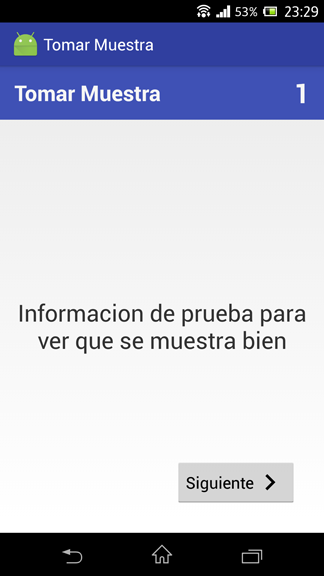
\includegraphics[scale=0.4]{05-implementacion/InformationStep.png} 
   \caption{Ejemplo de un InformationStep en ejecución}
   \label{fig:imgInformationStep}
\end{figure}

\subsubsection{InformationStepResult: El resultado de Mostrar información}
El resultado de mostrar información es nulo, es una clase vacía. Solo está para cerrar el circuito.

\subsection{PhotoStep: Tomar una foto}
PhotoStep se usa para solicitarle al científico ciudadano que tome una foto. Tiene un texto (instructionsToShow) que se muestran a modo de instrucciones o mensaje cuando la cámara esta encendida. Luego de tomada la foto, se muestra una vista preliminar de la misma, con un botón que da la opción de volver a tomar la foto.

En Android Studio (Java):
\begin{lstlisting}[language=Java, frame=tlb]	
PhotoStep step = new PhotoStep(1,"Por favor tome una foto de su gato",2);
\end{lstlisting}

Usando el generador de clases:
\begin{lstlisting}[language=XML, frame=tlb]	
{
  "id" : 1,
  "type" : "Photo",
  "text" : "Por favor tome una foto de su gato",
  "nextStepId" : 2
}
\end{lstlisting}

\begin{figure}[H]
  \centering
    
\includegraphics[scale=0.4]{05-implementacion/PhotoStep1.png} 
    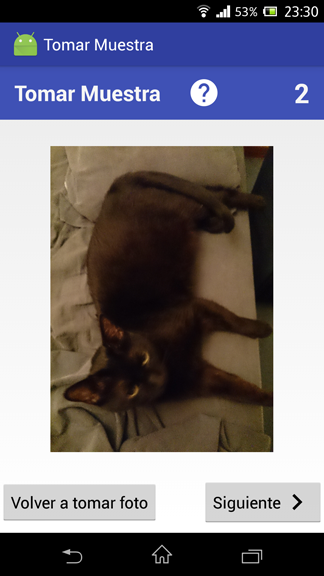
\includegraphics[scale=0.4]{05-implementacion/PhotoStep2.png}     
   \caption{Ejemplo de un PhotoStep en ejecución. A la izquierda al momento de tomar la foto, y a la derecha al momento de mostrar la vista preliminar.}
   \label{fig:imgPhotoStep}
\end{figure}

\subsubsection{PhotoStepResult: El resultado de Tomar una foto}
guarda el imageFileName de la foto. 
La foto va como archivo jpg en la carpeta de la muestra.
Puede haber varias fotos si hay varios PhotoSteps en el workflow

\subsection{SoundRecordStep: Grabar sonido}
Tiene instructionsToShow a modo de instrucciones que se muestran.

En Android Studio (Java):
\begin{lstlisting}[language=Java, frame=tlb]	
SoundRecordStep step = new SoundRecordStep(1,"Grabe el sonido de su auto",2); 
\end{lstlisting}

Usando el generador de clases:
\begin{lstlisting}[language=XML, frame=tlb]	
{
  "id" : 1,
  "type" : "Sound",
  "text" : "Grabe el sonido de su auto",
  "nextStepId" : 2
}
\end{lstlisting}

\subsubsection{SoundRecordStepResult: El resultado de Grabar sonido}
guarda el soundFileName del sonido.
El sonido va como archivo mp4 en la carpeta de la muestra.
Puede haber varios sonidos si hay varios SoundRecordSteps en el workflow


\subsection{SelectOneStep: Seleccionar una opción de un grupo de opciones}
Tiene un title
Las opciones son una lista de objetos SelectOneOption
Cada objeto SelectOneOption tiene un id, textToShow y nextStepId
Explicar la bifurcación de caminos en el workflow a partir de este Step
En forma de radio buttons

En Android Studio (Java):
\begin{lstlisting}[language=Java, frame=tlb]	
ArrayList<SelectOneOption> optionsToSelectOne = new ArrayList<SelectOneOption>();
optionsToSelectOne.add(new SelectOneOption(1,"Opcion 1", 2));
optionsToSelectOne.add(new SelectOneOption(2,"Opcion 2", 2));
optionsToSelectOne.add(new SelectOneOption(3,"Opcion 3", 3));
SelectOneStep step = new SelectOneStep(1,optionsToSelectOne,"Seleccione una opcion");

\end{lstlisting}

Usando el generador de clases:
\begin{lstlisting}[language=XML, frame=tlb]	
{
  "id" : 1,
  "type" : "SelectOne",
  "title" : "Seleccione una opcion",
  "options" : [
    {
      "id":1,
      "text":"Opcion 1",
      "nextStepId" : 2
    },
    {
      "id":2,
      "text":"Opcion 2",
      "nextStepId" : 2
    },
    {
      "id":3,
      "text":"Opcion 3",
      "nextStepId" : 3
    }
  ]
}
\end{lstlisting}

\subsubsection{SelectOneStepResult: El resultado de Seleccionar una opción de un grupo de opciones}
El resultado tiene la opción seleccionada (un objeto SelectOneOption)

\subsection{MultipleSelectStep: Seleccionar varias opciones de un grupo de opciones}
Tiene un title
Las opciones son una lista de objetos MultipleSelectOption
Cada objeto MultipleSelectOption tiene un id y textToShow
en forma de checkboxes

En Android Studio (Java):
\begin{lstlisting}[language=Java, frame=tlb]	
ArrayList<MultipleSelectOption> optionsToSelect = new ArrayList<MultipleSelectOption>();
optionsToSelect.add(new MultipleSelectOption(1,"Arboles"));
optionsToSelect.add(new MultipleSelectOption(2,"Basura"));
optionsToSelect.add(new MultipleSelectOption(3,"Agua"));
optionsToSelect.add(new MultipleSelectOption(4,"Animales"));
MultipleSelectStep step = new MultipleSelectStep(1,optionsToSelect,"Seleccione lo que ve",2); 
\end{lstlisting}

Usando el generador de clases:
\begin{lstlisting}[language=XML, frame=tlb]	
{
  "id" : 1,
  "type" : "MultipleSelect",
  "title" : "Seleccione lo que ve",
  "options" : [
    {
      "id":1,
      "text":"Arboles"
    },
    {
      "id":2,
      "text":"Basura"
    },
    {
      "id":3,
      "text":"Agua"
    },
    {
      "id":4,
      "text":"Animales"
    }
  ],
  "nextStepId" : 2
}
\end{lstlisting}

\subsubsection{MultipleSelectStepResult: El resultado de Seleccionar varias opciones de un grupo de opciones}
El resultado tiene una lista de las opciones seleccionadas (una lista de objetos MultipleSelectOption)



\subsection{LocationStep: Posicionar la muestra en el mapa con el GPS}
Tiene un textToShow a modo de instrucciones
Permite usar el GPS o posicionar la muestra manualmente en el mapa

En Android Studio (Java):
\begin{lstlisting}[language=Java, frame=tlb]	
LocationStep step = new LocationStep(1,"Por favor posicione la muestra en el mapa",2); 
\end{lstlisting}

Usando el generador de clases:
\begin{lstlisting}[language=XML, frame=tlb]	
{
  "id" : 1,
  "type" : "Location",
  "text" : "Por favor posicione la muestra en el mapa",
  "nextStepId" : 2
}
\end{lstlisting}

\subsubsection{LocationStepResult: El resultado de Posicionar la muestra en el mapa con el GPS}
Guarda latitude y longitude

\subsection{RouteStep: Grabar un recorrido en el mapa usando el GPS}
Tiene un textToShow a modo de instrucciones
Intervalo y mapZoom opcionales. Poner los valores por defecto

En Android Studio (Java):
\begin{lstlisting}[language=Java, frame=tlb]	
RouteStep step = new RouteStep(1,"Registre la ruta que corre",2); 
step.setInterval(10000);
step.setMapZoom(18);
\end{lstlisting}

Usando el generador de clases:
\begin{lstlisting}[language=XML, frame=tlb]	
{
  "id" : 1,
  "type" : "Route",
  "text" : "Registre la ruta que corre",
  "interval" : 10000,
  "mapZoom" : 18,
  "nextStepId" : 2
}
\end{lstlisting}

\subsubsection{RouteStepResult: El resultado de Grabar un recorrido en el mapa usando el GPS}
guarda una lista de objetos Location

\subsection{InsertTextStep: Ingresar texto}
textToShow a modo de instrucciones
sampleText a modo de ejmplo
maxLength cantidad máxima de caracteres permitida
Type Values allowed are: text, number or decimal
optional indicando si se puede dejar vacío y no ingresar ningún texto (true) o si se requiere que ingrese algo si o si (false)


En Android Studio (Java):
\begin{lstlisting}[language=Java, frame=tlb]	
InsertTextStep step = new InsertTextStep(1,"Por favor, ingrese el nombre del lago","Nombre del lago",50,InsertTextStep.InputType.TYPE_TEXT,true,2);
\end{lstlisting}

Usando el generador de clases:
\begin{lstlisting}[language=XML, frame=tlb]	
{
  "id" : 1,
  "type" : "InsertText",
  "text" : "Por favor, ingrese el nombre del lago",
  "sampleText" : "Nombre del lago",
  "inputType" : "text",
  "maxLength" : 50,
  "optional" : true,
  "nextStepId" : 2
}
\end{lstlisting}

\subsubsection{InsertTextStepResult: El resultado de Ingresar texto}
guarda el texto ingresado en insertedText

\subsection{InsertDateStep y InsertTimeStep: Ingresar fecha y hora}
ambos tienen textToShow a modo de instrucciones

En Android Studio (Java):
\begin{lstlisting}[language=Java, frame=tlb]	
InsertDateStep step = new InsertDateStep(1,"Por favor indique la fecha de la muestra",2); 
\end{lstlisting}

Usando el generador de clases:
\begin{lstlisting}[language=XML, frame=tlb]	
{
  "id" : 1,
  "type" : "InsertDate",
  "text" : "Por favor indique la fecha de la muestra",
  "nextStepId" : 2
}
\end{lstlisting}

En Android Studio (Java):
\begin{lstlisting}[language=Java, frame=tlb]	
InsertTimeStep step6 = new InsertTimeStep(1,"Por favor indique la hora de la muestra",2); 
\end{lstlisting}

Usando el generador de clases:
\begin{lstlisting}[language=XML, frame=tlb]	
{
  "id" : 1,
  "type" : "InsertTime",
  "text" : "Por favor indique la hora de la muestra",
  "nextStepId" : 2
}
\end{lstlisting}

\subsubsection{InsertDateStepResult y InsertTimeStep: El resultado de Ingresar fecha y hora}
un objeto Date que tiene la fecha o la hora según corresponda

\section{Mostrar Ayuda}

\section{Usando autenticación} \label{sec:usando_autenticacion}
Por defecto provee autenticación con Google, porque al tener Android tiene una cuenta de Google si o si.
Esta abierto a poder agregar autenticación con otras plataformas/APIs.

Samplers provee autenticación con Google, pero ese necesario registrar la aplicación en la pagina de desarrolladores de google (https://developers.google.com/identity/sign-in/android/start-integrating). Ahí hay que seguir los pasos para [to Configure a Google API Console project]. Es necesario [proveer] el nombre de la aplicación, package name, y también el SHA-1 hash del certificado con el que se firma la aplicación.

Una vez registrada la aplicación en Google, hay que configurar Samplers para habilitar la autenticación.

Una vez configurado los valores de los parámetros de autenticación, Samplers mostrará un fragment de inicio de sesión la primera vez que el usuario intente tomar una muestra. Si la autentición es opcional, se mostrará un botón para omitir el inicio de sesión y continuar con la toma de la muestra. También se muestra un botón para iniciar sesión en la activity principal (si se está usando la que provee Samplers).

Cuando la muestra es enviada, el id de usuario y el método de autenticación (por defecto 'google') se envían junto con esta.


\subsection{Configurar autenticación con el generador de clases de Gradle}

Para usar autenticación usando el generador de clases de Gradle, es necesario configurar los siguientes parámetros en el objeto \textbf{applicaction}:

\begin{itemize}

	\item \textbf{authenticationEnabled}: poner en true para habilitar la autenticación
		
	\item \textbf{authenticationOptional}: poner en true si se desea que la autenticación sea opcional, o en false si se desea que la autenticación sea obligatoria.
	
	\item Dentro del parámetro \textbf{networkConfiguration} es necesario establecer los parámetros \textbf{paramNameUserId} y \textbf{paramNameAuthenticationType} con los nombres de los parámetros con los que irán el id de usuario y el tipo de autenticación usada respectivamente dentro del mensaje HTTP POST.
	

\end{itemize}

Ejemplo:

\begin{lstlisting}[language=XML, frame=tlb]	
{
  "application": {
    "title" : "Samplers Hello World App",
    "welcomeMessage" : "Welcome to your first Samplers App!",
    "networkConfiguration" : {
      "url" : "http://192.168.1.10/samplers/upload.php",
      "paramName" : "sample",
      "paramNameUserId" : "user_id",
      "paramNameAuthenticationType" : "authentication_type"
    },
    "authenticationEnabled" : true,
    "authenticationOptional" : true
  } 
}
\end{lstlisting}

\subsection{Configurar autenticación [con instanciación manual]}

Para usar autenticación [con instanciación manual], es necesario definir la configuración de red y de autenticación en el método \textbf{onCreate()} de la activity principal:

\begin{lstlisting}[language=Java, frame=tlb]	
@Override
protected void onCreate(Bundle savedInstanceState) {
  super.onCreate(savedInstanceState);
	
  NetworkConfiguration.setURL("http://192.168.1.10/samplers/upload.php");
  NetworkConfiguration.setPARAM_NAME_SAMPLE("sample");
  // Set the authentication params of the Network Configuration
  NetworkConfiguration.setPARAM_NAME_USER_ID("user_id");
  NetworkConfiguration.setPARAM_NAME_AUTHENTICATION_TYPE("authentication_type");

  // Set the authenticationconfiguration
  AuthenticationManager.setAuthenticationEnabled(true);
  AuthenticationManager.setAuthenticationOptional(true);
}
\end{lstlisting}

\subsection{Usando un método de autenticación propio} \label{sec:usar_auth_propia}

Con Samplers también se puede usar un método de autenticación propio, definiendo un LoginFragment y una clase User (o varias clases si se desea proporcionar autenticación con diferentes APIs, como Facebook, Tweeter, Yahoo, etc.) y Samplers enviará junto con la muestra el id de usuario y el método de autenticación usado.


\subsubsection{Definiendo un Login Fragment [personalizado]}

Es necesario crear un fragment que herede de LoginFragment, y configurar la clase AuthenticationManager para que lo use, llamando al método setLoginFragmentClass() dentro del método onCreate() de la ativity principal:

\begin{lstlisting}[language=Java, frame=tlb]	
@Override
protected void onCreate(Bundle savedInstanceState) {
  super.onCreate(savedInstanceState);
	
  AuthenticationManager.setLoginFragmentClass(MyCustomLoginFragment.class);
}
\end{lstlisting}

El proceso de login y la interacción con las APIs responsabilidad del desarrollador, pero después de que el usuario inicia sesión en la API seleccionada, es necesario llamar al método login() en la clase AuthenticationManager y al método onLogin() en el objeto mListener heredado:

\begin{lstlisting}[language=Java, frame=tlb]	
if (loginOK) {
  AuthenticationManager.login(user, getActivity().getApplicationContext());
  mListener.onLogin(user);
}
\end{lstlisting}


\subsubsection{Definiendo una clase User [personalizada]}

Es necesario crear una clase usuario propia que implemente la interfaz User por cada método de autenticación que se use. Los objetos de dichas clases se usarán para llamar al método login() de la clase AuthenticationManager.

Ejemplo de una clase usuario propia:
\begin{lstlisting}[language=Java, frame=tlb]	
public class EMailUser implements User {

    public static final String AUTHENTICATION_TYPE = "email";

    private String userName;
    private String email;

    public GoogleUser(String userName, String email) {
        this.userName = userName;
        this.email = email;
    }

    @Override
    public String getAuthenticationType() {
        return AUTHENTICATION_TYPE;
    }

    @Override
    public String getUserName() {
        return userName;
    }

    @Override
    public String getUserId() {
        return email;
    }

}
\end{lstlisting}



\section{Personalización}

\subsection{Temas y colores}

\subsection{Idiomas}

\section{Definir un nuevo Step, StepFragment y StepResult ??} \label{sec:definir_steps}


